\documentclass[11pt,DIV=13,a4paper,abstract=true,twoside=semi,openright]
{scrreprt}
\usepackage[]{mathtools}
\usepackage[T1]{fontenc}
\usepackage[USenglish]{babel}
\usepackage[varqu,varl]{zi4}% inconsolata typewriter
% for lualatex
\usepackage{fontspec}
\setmonofont{Inconsolatazi4}
\usepackage{fontawesome5}
\usepackage{subcaption}
\usepackage[sfdefault,scaled=.85]{FiraSans}
\usepackage{sansmathaccent}
\ifnum 0\ifxetex 1\fi\ifluatex 1\fi=0 % if pdftex
\else % if luatex or xetex
  \usepackage{lualatex-math}
\fi
\usepackage{csquotes}
\usepackage{isabelle,isabellesym}
\usepackage{booktabs}
\usepackage{graphicx}
\usepackage{xspace}
\usepackage[cmyk]{xcolor}
\usepackage{listings}
\usepackage{railsetup}
\usepackage[backend=bibtex,style=trad-abbrv]{biblatex}
\addbibresource{root.bib}
\definecolor{lhWhite}        {RGB}{248,248,248}
\definecolor{lhOrange}       {RGB}{243,107, 33}
\definecolor{lhMagentaDark}  {RGB}{ 62, 10, 71}
\definecolor{CornflowerBlue}{cmyk}{0.65,0.13,0,0}

\usepackage[pdfpagelabels, pageanchor=false, plainpages=false]{hyperref}
\usepackage{orcidlink}
\newcommand\tocgobble[1]{}% 
%\renewcommand\familydefault{\sfdefault}
\colorlet{sectioncolor}{blue!60!black}
\addtokomafont{chapterentrypagenumber}{\color{sectioncolor}}
\addtokomafont{partentry}{\color{sectioncolor}\Large}
\addtokomafont{chapterentry}{\color{sectioncolor}}
\addtokomafont{title}{\color{sectioncolor}\bfseries}
\addtokomafont{part}{\color{sectioncolor}}
\addtokomafont{chapter}{\color{sectioncolor}\bfseries}
\addtokomafont{section}{\color{sectioncolor}}
\addtokomafont{subsection}{\color{sectioncolor}}
\addtokomafont{subsubsection}{\color{sectioncolor}}
\addtokomafont{paragraph}{\color{sectioncolor}}
\addtokomafont{subparagraph}{\color{sectioncolor}}
\sloppy

\addtokomafont{partentry}{\hfill}
\RedeclareSectionCommand[
  tocpagenumberbox=\tocgobble%
]{part}


\renewcommand{\isastyletext}{\normalsize\normalfont\sffamily}
\renewcommand{\isastyletxt}{\normalfont\sffamily}
\renewcommand{\isastylecmt}{\normalfont\sffamily}
%e% This is a placeholder for user-specific configuration and packages.
\usepackage{textcomp}
\usepackage{xcolor}
\usepackage{paralist}
\usepackage[en-US]{datetime2}      % For \DTMdate, etc.
\usepackage{amssymb}
\usepackage{listings}
\usepackage{lstisadof}
\usepackage{xspace}
\usepackage[draft]{fixme}
\usepackage{wrapfig}

\addauthor{\href{https://www.lri.fr/~ftuong/}{Frédéric Tuong}\inst{1} \and \href{https://www.lri.fr/~wolff/}{Burkhart Wolff}\inst{1}} % should be auto-generated

\newcommand{\house}{\mathrel{\substack{\wedge\\[-.2em]\sqcup}}}

\isabellestyle{literal}
\isabellestyle{tt}
\usepackage{listings}
\usepackage{listingsutf8}
\usepackage[many]{tcolorbox}
\tcbuselibrary{listings}
\tcbuselibrary{skins}

\lstdefinelanguage{JSON}{%
  keywords={},
  keywordstyle=\color{blue}\bfseries,
  ndkeywords={},
  ndkeywordstyle=\color{darkgray}\bfseries,
  identifierstyle=\color{black},
  sensitive=false,
  comment=[l]{//},
  morecomment=[s]{/*}{*/},
  % ommentstyle=\color{purple}\ttfamily,
%  stringstyle=\color{red}\ttfamily,
  morestring=[b]',
  morestring=[b]"
}
\lstdefinestyle{json}{language=JSON,
  basicstyle=\ttfamily\color{black},
  commentstyle=\itshape\color{black},
  stringstyle=\color{lhOrange},
  keywordstyle=\color{lhCyan},
  ndkeywordstyle=\color{lhGreen},
}
\lstdefinestyle{displayjson}{style=json,
  floatplacement={tbp},
  captionpos=b,
  framexleftmargin=0pt,
  basicstyle=\ttfamily\color{black},
  numbers=left,,%=left,
  numberstyle=\footnotesize,
  stepnumber=1,
  backgroundcolor=\color{black!95},
  frame=lines,
  xleftmargin=1cm,
  escapeinside={(*@}{@*)}
}

\def\inlinejson{\lstinline[style=json, columns=fullflexible]}
\newtcblisting{json}[1][]{%
      listing only%
     ,boxrule=0pt
     ,boxsep=0pt
     ,colback=white!90!gray
     ,enhanced jigsaw
     ,borderline west={2pt}{0pt}{gray!60!black}
     ,sharp corners
     % ,before skip=10pt
     % ,after skip=10pt
     ,enlarge top by=0mm
     ,enhanced
     ,overlay={\node[draw,fill=gray!60!black,xshift=0pt,anchor=north
       east,font=\bfseries\footnotesize\color{white}]
                at (frame.north east) {JSON};}
        ,listing options={
          style=json
          ,breakatwhitespace=true
          ,columns=flexible%
          ,basicstyle=\small\ttfamily
          %,mathescape
          ,#1
      }
  }%

%%%%%%%%%%%%%%%%%%%%%%%%%%%%%%%%%%%%%%%%%%%%%%%%%%%%%%%%%%%%%%%%%%%%%%%%%%%%%% 
%% <python>
\lstloadlanguages{python}
\providecolor{python}{named}{lhMagentaDark}
\lstdefinestyle{python}{
   basicstyle=\ttfamily,%
   commentstyle=\itshape,%
   keywordstyle=\bfseries\color{CornflowerBlue},%
   ndkeywordstyle=\color{green},%
   language=python
   ,keywordstyle=[6]{\itshape}%
   ,morekeywords=[6]{args_type}%
}%
\def\inlinepython{\lstinline[style=python,breaklines=true,mathescape,breakatwhitespace=true]}
\newtcblisting{python}[1][]{%
      listing only%
     ,boxrule=0pt
     ,boxsep=0pt
     ,colback=white!90!python
     ,enhanced jigsaw
     ,borderline west={2pt}{0pt}{python!60!black}
     ,sharp corners
     % ,before skip=10pt
     % ,after skip=10pt
     ,enlarge top by=0mm
     ,enhanced
     ,overlay={\node[draw,fill=python!60!black,xshift=0pt,anchor=north
       east,font=\bfseries\footnotesize\color{white}]
                at (frame.north east) {Python};}
        ,listing options={
          style=python
          ,columns=flexible%
          ,basicstyle=\small\ttfamily
          ,mathescape
          ,#1
      }
  }%
%% </python>
%%%%%%%%%%%%%%%%%%%%%%%%%%%%%%%%%%%%%%%%%%%%%%%%%%%%%%%%%%%%%%%%%%%%%%%%%%%%%% 


%%% <todo>
\usepackage{tcolorbox}
\isakeeptag{todo}
\newenvironment{isatodoenv}{%
\mbox{}\\
\tcbsetforeverylayer{colframe=red!75!black}
\begin{tcolorbox}[title={\textsf{\textbf{ToDo}}}]}{%
\end{tcolorbox}
}
\renewcommand{\isatagtodo}{\begin{isatodoenv}}
\renewcommand{\endisatagtodo}{\end{isatodoenv}}
%%% </todo>
\isabellestyle{literal}
\isabellestyle{it}
\renewcommand{\isacharunderscore}{\_}%
\renewcommand{\isacharunderscorekeyword}{\_}%

\newcommand{\thy}{%
  \begingroup% 
    \def\isacharunderscore{\textunderscore}%
    {\small\faFile*[regular]}\,\isabellecontext%
  \endgroup% 
}

\renewcommand{\isamarkupchapter}[1]{\chapter{#1 (\thy)}}
\let\oldisakeyword\isakeyword
\renewcommand{\isakeyword}[1]{\oldisakeyword{\color{black!70!white}#1}}
\renewcommand{\isacommand}[1]{\isakeyword{\color{sectioncolor}#1}}

\usepackage{hyperref}
\urlstyle{sf}
\setcounter{tocdepth}{2} 
\hypersetup{%
   bookmarksdepth=3
  ,pdfpagelabels
  ,pageanchor=true
  ,bookmarksnumbered
  ,plainpages=false
} % more detailed digital TOC (aka bookmarks)

\begin{document}
\renewcommand{\chapterautorefname}{Chapter}
\renewcommand{\sectionautorefname}{Section}
\renewcommand{\subsectionautorefname}{Section}
\renewcommand{\subsubsectionautorefname}{Section}
\maketitle
\begin{abstract}
  \begin{quote}
    Interval analysis (also called interval arithmetic) is a well known
    mathematical technique to analyse or mitigate rounding errors or measurement
    errors. Thus, it is promising to integrate interval analysis into program
    verification environments. Such an integration is not only useful for the
    verification of numerical algorithms: the need to ensure that computations
    stay within certain bounds is common. For example to show that computations
    stay within the hardware bounds of a given number representation.
  
    Another application is the verification of cyber-physical systems, where a
    discretised implementation approximates a system described in physical
    quantities expressed using perfect mathematical reals, and perfect ordinary
    differential equations.
  
    In this AFP entry, we formalise extended interval analysis,  including the
    concept of inclusion isotone (or inclusion isotonic) (extended) interval analysis. The main result
    is the formal proof that interval-splitting converges for Lipschitz-continuous 
    interval isotone functions. From pragmatic perspective, we provide the 
    datatypes and theory required for integrating interval analysis into
    other formalisations and applications. 
    
  \bigskip
  \noindent\textbf{Keywords:} Extended Interval Analysis, Formalising Mathematics, Isabelle/HOL
  \end{quote}
\end{abstract}

\tableofcontents

\chapter{Introduction}
Interval analysis~\cite{moore.ea:introduction:2009} in general and, in
particular, inclusion isotone extended interval
arithmetic~\cite{ratz:inclusion:1997} are  well known mathematical techniques to
analyse or mitigate rounding errors or measurement errors. Thus, it is promising to
integrate interval analysis into program verification environments. Such an
integration is not only useful for the verification of numerical algorithms:
the need to ensure that computations stay within certain bounds is common.
For example to show that computations stay within the hardware bounds of
a given number representation.

Another application is the verification of cyber-physical systems, were a
discretised implementation approximates a system described in physical
quantities expressed using perfect mathematical reals, and perfect ordinary
differential equations.  Moreover, first applications of interval analysis to the
security analysis of neural networks are
promising~\cite{wang.ea:formal-security:2018,harapanahalli.ea:toolbox:2023} and, 
when combined with existing works of verifying neural networks in 
Isabelle~\cite{brucker.ea:feedforward-nn-verification:2023} provide a verification 
approach using a ``correct-by-construction'' verification tool for neural networks. 

In this AFP entry, we formalise extended interval analysis,  including the
concept of inclusion isotone (extended) interval analysis. The main result
is the formal proof that interval-splitting converges for Lipschitz-continuous 
inclusion isotone functions. From pragmatic perspective, we provide the 
datatypes and theory required for integrating interval analysis into
other formalisations and applications.  In more detail, our contributions
are:
\begin{enumerate}
  \item a conservative formalisation of (extended) interval arithmetic in
  Isabelle/HOL, including inclusion isotonicity;
  \item we formally prove that interval-splitting converges for
  Lipschitz-continuous inclusion isotone functions;
\end{enumerate}

From an end-user's perspective, the main entry points into this session 
are the following three theories:
\begin{itemize}
\item \texttt{Interval\_Analysis} (\autoref{cha:interval_analysis}):
      This theory provides interval analysis over standard types such as real or integer. All operations 
      work over (closed) intervals. 
\item \texttt{Extended\_Interval\_Analysis} (\autoref{cha:extended_interval_analysis}):
      This theory provides extended interval analysis over the type extended reals. All operations 
      work over (closed) intervals.
\item \texttt{Extended\_Multi\_Interval\_Analysis} (\autoref{cha:extended_multi_interval_analysis}):
      This theory provides extended multi-interval analysis over the type extended reals. All operations 
      work over multi-intervals, i.e., lists of (closed) intervals. 
\end{itemize}

The following publication~\cite{brucker.ea:formally:2024} gives a high-level overview of this AFP entry:
\begin{quote}
  A. D. Brucker, T. Cameron-Burke, and A. Stell. Formally verified interval arithmetic and its application to
  program verification. In 13th IEEE/ACM International Conference on Formal Methods in Software Engineering 
  (FormaliSE 2024). IEEE, 2024.
\end{quote} 

\begin{figure}
  \centering
  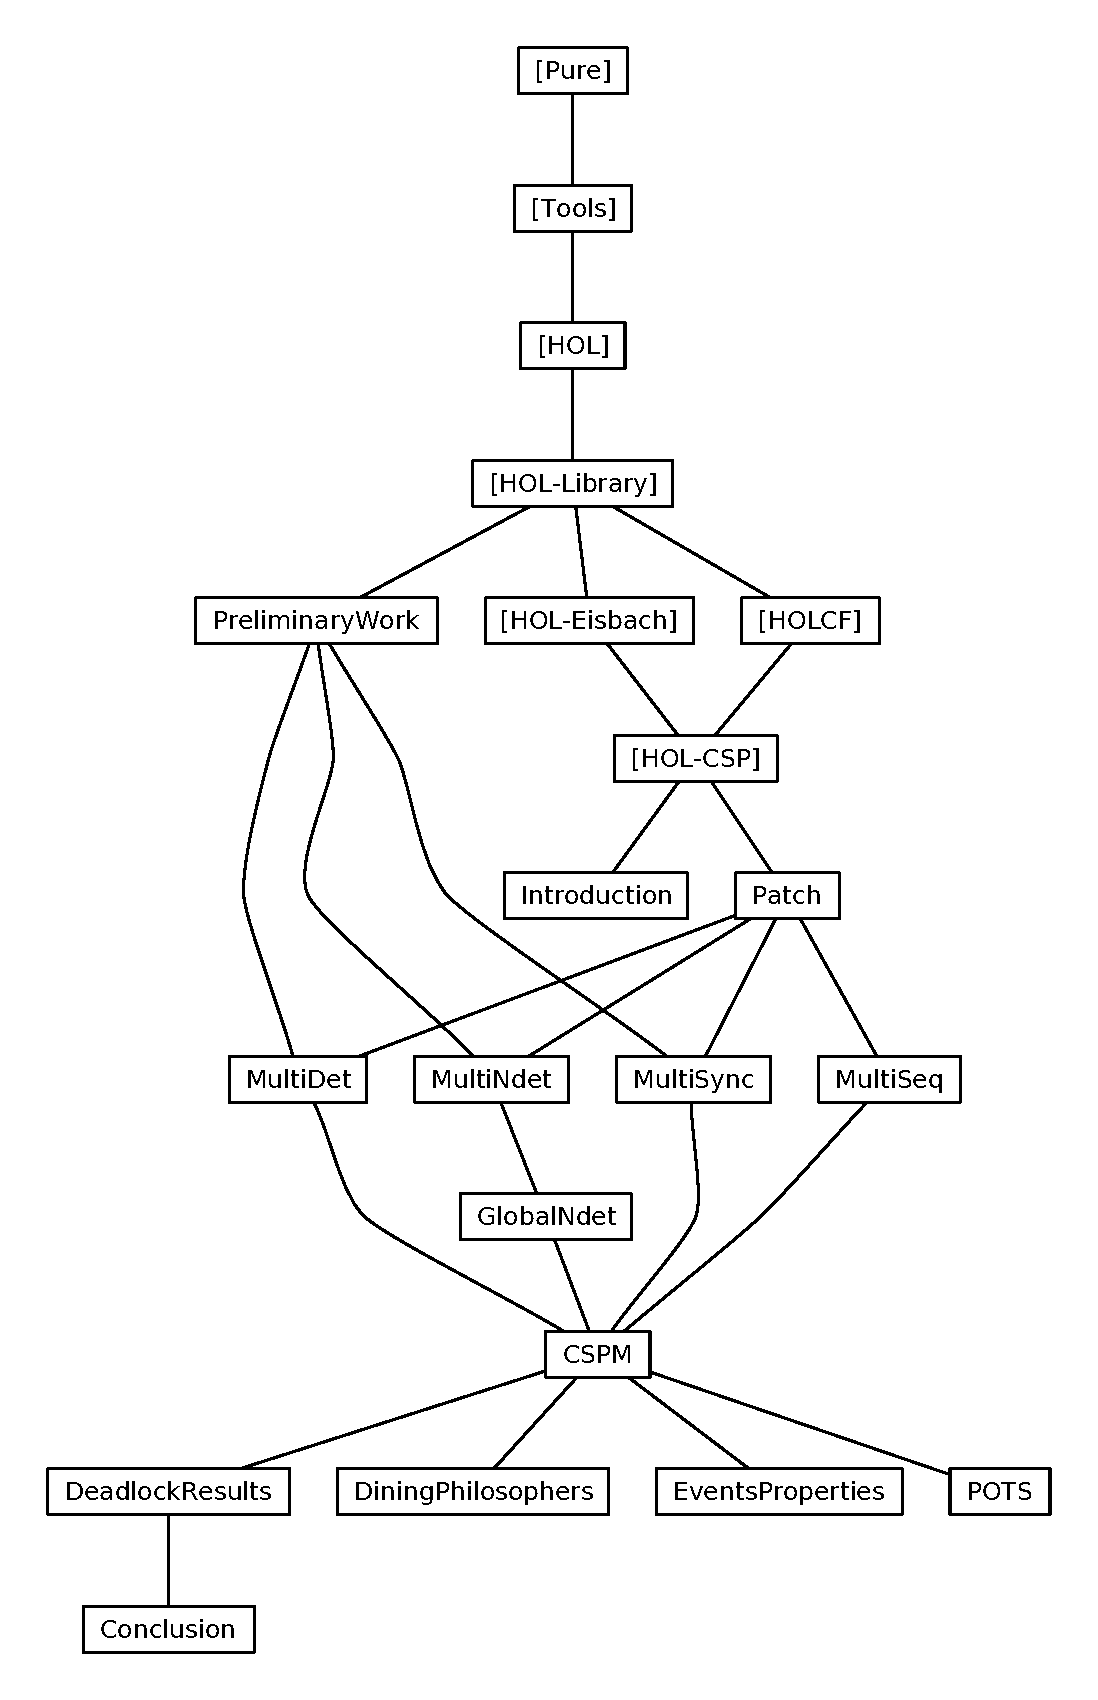
\includegraphics[height=\textheight, width=\textwidth, keepaspectratio]{session_graph}
  \caption{The Dependency Graph of the Isabelle Theories.\label{fig:session-graph}}
\end{figure}
The rest of this document is automatically generated from the
formalisation in Isabelle/HOL, i.e., all content is checked by
Isabelle.  Overall, the structure of this document follows the
theory dependencies (see \autoref{fig:session-graph}). 

\part*{Generated Sessions}
\input{session}
\printbibliography
\end{document}

%%% Local Variables:
%%% mode: latex
%%% TeX-master: t
%%% End:
\endinput
